\section{Metodología}

\subsection{Descripción de los datos}
Se dispone de dos archivos. El primero, \texttt{set\_cover\_500x500.csv}, es una matriz de $500\times 500$ con valores 0 y 1, donde la entrada de la fila $i$ y la columna $j$ vale 1 si la antena ubicada en $j$ cubre al cliente $i$. El segundo, \texttt{Costo\_S.xlsx}, contiene el costo de instalación de cada una de las 500 antenas.

La matriz tiene una densidad de 0,0999, es decir, cerca del 10\,\% de las entradas son unos. Cada cliente queda cubierto por entre 32 y 70 antenas, y cada antena cubre entre 33 y 66 clientes. Los costos van de 2\,000 a 3\,998, con un promedio de 3\,033,6. La Figura~\ref{fig:datos} muestra la distribución de los costos y de la cobertura por cliente. Como todo cliente tiene al menos 32 antenas que lo cubren, la instancia es factible (por ejemplo, instalando todas las antenas).

\begin{figure}[H]
\centering
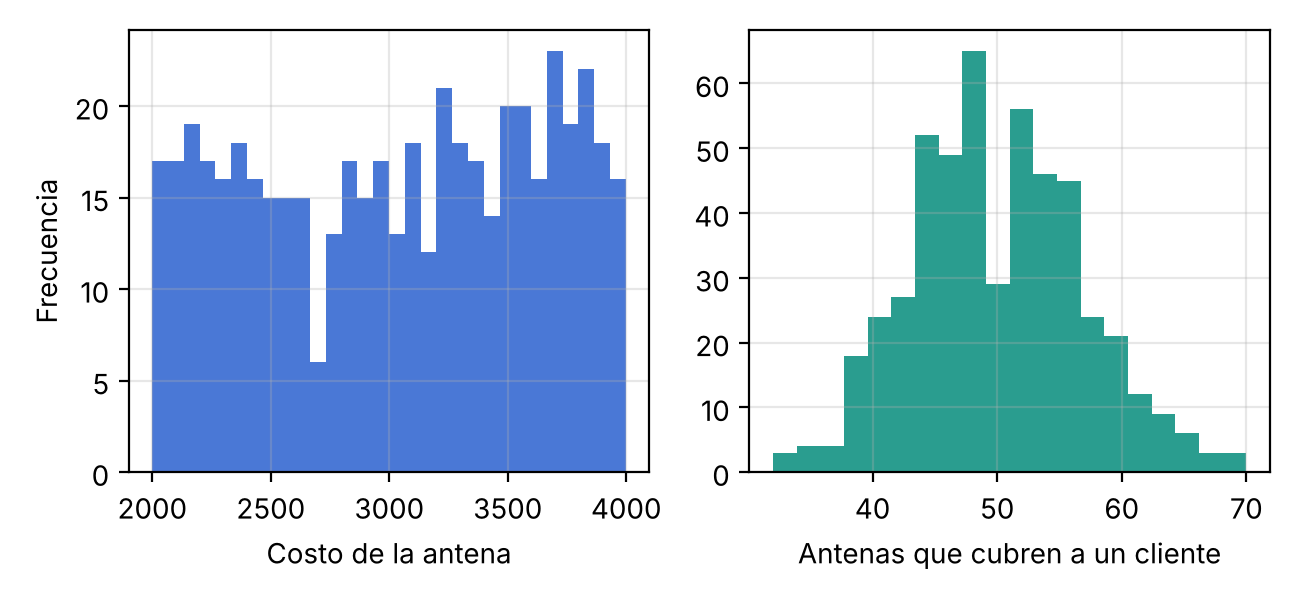
\includegraphics[width=0.85\textwidth]{figuras/datos.png}
\caption{Distribución de los costos de las antenas y del número de antenas que cubren a cada cliente.}
\label{fig:datos}
\end{figure}

\subsection{Formulación matemática}

\paragraph{Conjuntos e índices.}
$I=\{1,\dots,500\}$ es el conjunto de clientes, indexado por $i$; $J=\{1,\dots,500\}$ es el conjunto de ubicaciones de antenas, indexado por $j$.

\paragraph{Parámetros.}
\begin{itemize}
\item $a_{ij}\in\{0,1\}$: vale 1 si la antena $j$ cubre al cliente $i$ y 0 en caso contrario.
\item $c_j>0$: costo de instalar la antena $j$.
\end{itemize}

\paragraph{Variables de decisión.}
\[
x_j=\begin{cases}1 & \text{si se instala una antena en la ubicación } j,\\ 0 & \text{en caso contrario,}\end{cases}\qquad j\in J.
\]

\paragraph{Modelo.}
\begin{align}
\min\; Z &= \sum_{j\in J} c_j\,x_j \label{eq:obj}\\
\text{s.a.}\quad \sum_{j\in J} a_{ij}\,x_j &\ge 1 \qquad \forall\, i\in I \label{eq:cob}\\
x_j &\in\{0,1\} \qquad \forall\, j\in J \label{eq:bin}
\end{align}

\paragraph{Significado de cada componente.}
La función objetivo \eqref{eq:obj} es el costo total de las antenas instaladas, que se desea minimizar. Las restricciones \eqref{eq:cob} garantizan la cobertura: para cada cliente $i$, la suma $\sum_j a_{ij}x_j$ cuenta cuántas antenas instaladas lo cubren, y debe ser al menos 1. Las restricciones \eqref{eq:bin} indican que cada ubicación se usa o no se usa; no se pueden instalar fracciones de antena. El modelo tiene 500 variables binarias y 500 restricciones de cobertura.

\subsection{Solución exacta}
El modelo \eqref{eq:obj}--\eqref{eq:bin} se implementó en Python y se resolvió con el solver HiGHS \cite{highs18} mediante la función \texttt{scipy.optimize.milp}. Se fijó un límite de tiempo de 600 segundos y una brecha relativa de optimalidad de 0. Se registraron el costo de la mejor solución entera, la cota inferior del solver, la brecha entre ambos y el tiempo de cómputo.

\subsection{Algoritmo Genético}

\paragraph{Codificación.}
Cada individuo es un vector binario $\mathbf{x}=(x_1,\dots,x_{500})$ con la misma interpretación que las variables del modelo: $x_j=1$ si se instala la antena $j$.

\paragraph{Reparación.}
Dado un vector $\mathbf{x}$ cualquiera, se aplica el procedimiento de reparación de dos fases, inspirado en Beasley y Chu \cite{beasley96}:
\begin{enumerate}
\item \textbf{Fase de cobertura:} mientras haya clientes sin cubrir, se agrega la antena que minimiza la razón $c_j / n_j$, donde $n_j$ es el número de clientes sin cubrir que la antena $j$ cubriría. Esto es el criterio voraz de Chv\'atal \cite{chvatal79}.
\item \textbf{Fase de eliminación de redundancias:} se recorren las antenas instaladas de la más cara a la más barata y se elimina cada una cuya salida deje a todos sus clientes con al menos otra antena.
\end{enumerate}

\paragraph{Fitness.}
Como todo individuo reparado es factible, el fitness es simplemente el costo $f(\mathbf{x})=\sum_j c_jx_j$, que se minimiza.

\paragraph{Inicialización.}
Cada individuo de la población inicial se genera activando cada gen con probabilidad $p_{\text{init}}=0{,}05$ y reparando el resultado. Esto produce individuos diversos y factibles desde el comienzo.

\paragraph{Selección.}
Se usa selección por torneo de tamaño $k=3$: se toman $k$ individuos al azar y se elige el de menor costo.

\paragraph{Cruce.}
Con probabilidad $p_c=0{,}9$, los dos padres se combinan mediante cruce uniforme: cada gen del hijo se toma de un padre u otro con probabilidad $1/2$. Con probabilidad $1-p_c$ el hijo es copia del primer padre.

\paragraph{Mutación.}
Cada gen del hijo se invierte de forma independiente con probabilidad $p_m=1/n=0{,}002$, de modo que en promedio se muta un gen por hijo. Tras la mutación el hijo se repara.

\paragraph{Elitismo y criterio de parada.}
Los 2 mejores individuos pasan sin cambios a la siguiente generación. El algoritmo se detiene al llegar a 300 generaciones o cuando el mejor costo no mejora durante 80 generaciones consecutivas.

\paragraph{Parámetros.}
La Tabla~\ref{tab:params} resume los parámetros de la configuración base y las variantes que se estudiaron.

\begin{table}[H]
\centering
\caption{Parámetros del Algoritmo Genético.}
\label{tab:params}
\begin{tabular}{lcccc}
\toprule
Parámetro & Base & Población pequeña & Población grande & Mutación alta\\
\midrule
Tamaño de población & 100 & 30 & 300 & 100\\
Probabilidad de cruce & 0,9 & 0,9 & 0,9 & 0,9\\
Probabilidad de mutación por gen & $1/500$ & $1/500$ & $1/500$ & $5/500$\\
Tamaño del torneo & 3 & 3 & 3 & 3\\
Élite & 2 & 2 & 2 & 2\\
Máx. generaciones & 300 & 300 & 300 & 300\\
Paciencia (generaciones) & 80 & 80 & 80 & 80\\
\bottomrule
\end{tabular}
\end{table}

\begin{algorithm}[H]
\caption{Algoritmo Genético con reparación para el Set Cover}
\begin{algorithmic}[1]
\State Generar población inicial de $N$ individuos y repararlos
\State Evaluar el costo de cada individuo
\For{$g=1,\dots,G_{\max}$}
  \State Copiar los $E$ mejores individuos a la nueva población (elitismo)
  \While{la nueva población tenga menos de $N$ individuos}
    \State Seleccionar dos padres por torneo
    \State Con probabilidad $p_c$ aplicar cruce uniforme; si no, copiar el primer padre
    \State Mutar cada gen con probabilidad $p_m$
    \State Reparar el hijo y agregarlo a la nueva población
  \EndWhile
  \State Evaluar la nueva población y actualizar la mejor solución
  \If{no hubo mejora en $P$ generaciones} \State \textbf{parar} \EndIf
\EndFor
\State \Return mejor solución encontrada
\end{algorithmic}
\end{algorithm}

\subsection{Diseño experimental}
Los algoritmos se implementaron en Python con NumPy y SciPy \cite{scipy20}. El AG es estocástico, por lo que un único resultado no es representativo: cada configuración de la Tabla~\ref{tab:params} se ejecutó 10 veces con semillas distintas (0 a 9). Se registraron el costo final, el número de antenas, el número de generaciones y el tiempo de cómputo. Además se ejecutó una configuración \textit{extendida} (población de 200, mutación $2/n$, hasta 3\,000 generaciones y paciencia de 400) con otras 10 semillas, para estudiar el efecto de una búsqueda más larga. Como referencias adicionales se calcularon la heurística voraz de Chv\'atal y la cota inferior de la relajación lineal. Para comparar con el método exacto se calculó la brecha relativa
\[
\text{Brecha}=\frac{Z_{\text{AG}}-Z_{\text{ref}}}{Z_{\text{ref}}}\times 100\,\%,
\]
donde $Z_{\text{ref}}$ es el costo de la mejor solución entera del solver exacto.

\subsection{Interfaz visual}
Se desarrolló una aplicación web con Streamlit que permite cargar los datos, ejecutar el solver exacto y el AG con parámetros ajustables, ver las curvas de convergencia y comparar ambos métodos en costo, tiempo y antenas seleccionadas.
